\PassOptionsToPackage{utf8}{inputenc}
\documentclass{bioinfo}
\copyrightyear{2015} \pubyear{2015}

\access{Advance Access Publication Date: Day Month Year}
\appnotes{Manuscript Category}


% Notes

% Citation styles:
% \cite:    Foo et al. (2018)
% \citep:   (Foo et al., 2018)
% \citealp: Foo et al., 2018

% Equations:
% use \begin{equation}

% Tables:
% \begin{table}[!t]
% \processtable{This is table caption\label{Tab:01}}
% {\begin{tabular}{@{}llll@{}}\toprule head1 &
% head2 & head3 & head4\\\midrule
% row1 & row1 & row1 & row1\\
% row2 & row2 & row2 & row2\\
% row3 & row3 & row3 & row3\\
% row4 & row4 & row4 & row4\\\botrule
% \end{tabular}}{This is a footnote}
% \end{table}

% Figures:
% \begin{figure}[!tpb]%figure2
% \centerline{\includegraphics{fig02.eps}}
% \caption{Caption, caption.}\label{fig:02}
% \end{figure}

% Sectioning:
% use \section, \subsection, \subsubsection (numbered non-star version)

% The submission page (https://academic.oup.com/bioinformatics/pages/instructions_for_authors) says we should use:
% Introduction, System and methods, Algorithm, Implementation, Discussion, References
% The template has:
% Introduction, Approach, Methods, Discussion, Conclusion
% But recently published articles show this:
% Introduction, Materials and methods, Results, Discussion (https://doi.org/10.1093/bioinformatics/bty179, .../bty193, .../bty117)


% The template wraps parts of the Methods section in \begin{methods} --
% why? why only parts of it?

% Template uses \enlargethispage{12pt}
% Template uses \vadjust{\newpage} and \vadjust{\pagebreak} (what do they do?)


\newcommand{\url}[1]{\href{#1}{#1}}
\newcommand{\eg}{e.\,g.\ }
\newcommand{\ie}{i.\,e.\ }


\begin{document}
\firstpage{1}

\subtitle{Data and text mining}

\title[Context-aware disease linking]{Context-aware disease linking}
\author[Sample \textit{et~al}.]{Corresponding Author\,$^{\text{\sfb 1,}*}$, Co-Author\,$^{\text{\sfb 2}}$ and Co-Author\,$^{\text{\sfb 2,}*}$}
\address{$^{\text{\sf 1}}$Department, Institution, City, Post Code, Country and \\
$^{\text{\sf 2}}$Department, Institution, City, Post Code,
Country.}

\corresp{$^\ast$To whom correspondence should be addressed.}

\history{Received on XXXXX; revised on XXXXX; accepted on XXXXX}

\editor{Associate Editor: XXXXXXX}


\abstract{%
\textbf{Motivation:} This section should specifically state the scientific question within the context of the field of study.\\
\textbf{Results:} This section should summarize the scientific advance or novel results of the study, and its impact on computational biology.\\
\textbf{Availability and Implementation:} This section should state software availability if the paper focuses mainly on software development or on the implementation of an algorithm. Examples are: 'Freely available on the web at \url{http://www.example.org}'; 'Website implemented in Perl, MySQL and Apache, with all major browsers supported'; or 'Source code and binaries freely available for download at URL, implemented in C++ and supported on linux and MS Windows'. The complete address (URL) should be given. If the manuscript describes new software tools or the implementation of novel algorithms the software must be freely available to non-commercial users. Authors must also ensure that the software is available for a full TWO YEARS following publication. The editors of Bioinformatics encourage authors to make their source code available and, if possible, to provide access through an open source license (see www.opensource.org for examples).\\
\textbf{Contact:} Full email address to be given, preferably an institution email address.\\
\textbf{Supplementary information:} Links to additional figures/data available on a web site, pr reference to online-only supplementary data available at the journal's web site.
}

\maketitle

\section{Introduction}

introduce task (linking vs. NER)

discuss state of the art (nobody uses context!)



\section{Materials and methods}

\subsection{Datasets}

We evaluated the proposed system using two annotated document collections.
The ShARe corpus consists of clinical reports with annotations for diseases and disorders, which were created for the ShARe/CLEF eHealth Evaluation Lab 2013 shared task \citep{pradhan-et-al:2013:CLEF}.
The NCBI disease corpus \citep{islamaj-dogan-et-al:2014} provides disease annotations over abstracts of scientific articles.
Both collections include references to the relevant mentions in their original context and link them to identifiers of a standard knowledge base.
In both cases, a predefined division into training and test set allows comparison across different approaches.
More detailed statistics on the datasets are given in Table~\ref{tab:datasets}.

The ShARe corpus contains de-identified clinical reports from US intensive care.
It is distributed as part of the MIMIC database  % TODO: reference
and is available for research purposes after acquiring a personal license.%
\footnote{Instructions for obtaining the data are given on the shared-task website, currently hosted at \url{https://sites.google.com/site/shareclefehealth/data}.}
The annotated mentions are grounded in the SNOMED CT terminology  % TODO: reference
using UMLS  % TODO: reference
identifiers (CUI).
Concepts that were not represented in SNOMED at the time of annotation were given the NIL symbol “CUI-less”.

The NCBI disease corpus comprises scientific abstracts and annotations which are freely available online.
In addition to the training and test set, a predetermined development set is provided (regarded as part of the training set in Table~\ref{tab:datasets}).
The mentions are linked to the MEDIC vocabulary  % TODO: reference
using MeSH  % TODO: reference
and OMIM  % TODO: reference
identifiers.
Unlike the ShARe corpus, the NCBI annotators were required to always provide an identifier, \ie there is no NIL label.
Furthermore, they were asked to map a mention to multiple identifiers if there was no single terminology entry that sufficiently covered the meaning of the concept in question.
As another difference, composite mentions such as “breast and ovarian cancer” are represented as a single annotation with a series of identifiers, whereas the ShARe corpus uses multiple, partially overlapping annotations (“breast [\dots] cancer” and “ovarian cancer”).

\begin{table}[!t]
\processtable{Dataset statistics.\label{tab:datasets}}
{\begin{tabular}{@{}lrr@{}}\toprule
              & NCBI disease corpus$^\text{\sfb 1}$ & ShARe corpus\\\midrule
  documents   & 792     & 298\\
  ./. testset & 100+100 & 99\\
  words       & 153394  & 177452\\
  mentions    & 6881    & 11167\\
  concepts    & 790     & 1354\\
  \midrule
  vocabulary  & MEDIC   & SNOMED-CT\\
  concepts    & 9664    & 72368\\
  synonyms    & 67784   & 198371\\
  \botrule
\end{tabular}}{$^\text{\sfb 1}$The figures differ slightly from the ones reported by \cite{islamaj-dogan-et-al:2014} because the training set contains a duplicate document (PMID 8528200), which we counted only once.}
\end{table}

% TODO: describe addition of UMLS synonyms (different strategy for ShARe and NCBI, incl. usage of NIL label)


\subsection{System architecture}

We approach the entity linking task in a three-stage process:
generating candidate names (Section~\ref{ssub:cand-gen}),
ranking candidates (\ref{ssub:ranking}), and
mapping names to identifiers (\ref{ssub:id-mapping}).
In the candidate-generation stage, different strategies are used to extract a selection of synonyms from the knowledge base for each mention.
For the second stage, a CNN is trained to assign a score to each proposed mention-synonym pair.
In the last stage, the scored list is examined to pick the most likely identifier for each mention.

\subsubsection{Candidate generation}
\label{ssub:cand-gen}

The candidate generation phase is a preprocessing step for the subsequent ranking task.
It aims at keeping the ranking lists at a manageable size without missing relevant names.
A good recall value is crucial for the candidate generation, as it poses a hard upper boundary on the entire pipeline.

We implemented a candidate generator based on orthographic similarity, another one on semantic similarity, and a number of ancillary generators targeting specific cases.
For the orthographic similarity, mentions and candidates are represented as vectors of their character skip-grams (\ie n-grams with gaps),  % TODO: reference
which allows efficient computation of pair-wise cosine similarity.
The shape of the skip-grams, a similarity threshold as well as a cut-off value are experimental parameters that control the number of candidates returned for each mention.
For the semantic similarity, mentions and candidates are represented as phrase vectors, which are obtained by averaging over the word vectors of pretrained embeddings.
The most similar candidates are determined through pair-wise cosine, analogously to the orthographic similarity.
The ancillary generators are concerned with specific tasks like abbreviation expansion, digit/numeral replacement, hyperonym relation, and composite mentions.
They operate in their respective niche and are triggered only in certain circumstances.
Table~\ref{tab:candidate-generation} illustrates candidate generation with an example.

The generators provide a score for each candidate.
The cosine-based generators return a value in the range $[0,1]$, while others report $1$ for every candidate they can find.
If multiple generators produced the same candidate, their scores are aggregated; a $0$ score is substituted for each generator that did not produce the candidate in question.
For each candidate, a vector of scores is provided to the CNN, along with the candidate name.

oracle mode!

\begin{table}[!t]
\processtable{Candidate names generated for the mention ``fragile X syndrome'' (selected output with scores for the orthographic, semantic, and hyperonym generation strategy)\label{tab:candidate-generation}}
{\begin{tabular}{@{}llll@{}}\toprule
  Candidate name & orth. sim. & sem. sim. & hyp.\\\midrule
  Fragile X Syndrome                             & 1      & 1      & --\\
  Fragile X Syndromes                            & 0.9698 & 1      & --\\
  fragile syndrome x                             & 0.8376 & 0.9431 & --\\
  Syndrome, Fragile X                            & 0.7765 & 1      & --\\
  FRAXA - Fragile X syndrome                     & 0.8355 & 0.9380 & --\\
  Syndrome                                       & 0.6059 & --     & 1 \\
  Five X syndrome                                & 0.7172 & 0.8800 & --\\
  Trisomy X syndrome                             & --     & 0.8567 & --\\
  fragile-x syndrome                             & 0.8354 & --     & --\\
  Syndrome, FRAXA                                & --     & 0.8350 & --\\
  XXXXX syndrome                                 & --     & 0.8109 & --\\
  X Linked Mental Retardation and Macroorchidism & --     & 0.8022 & --\\
  Alagille Syndrome                              & 0.6506 & --     & --\\
  XXX syndrome                                   & 0.5721 & --     & --\\
  \botrule
\end{tabular}}{}
\end{table}

\subsubsection{Ranking}
\label{ssub:ranking}

For ranking the candidate names created in the previous step, we trained a CNN similar to the approach reported by \cite{lihaodi-et-al:2017}.
Key differences are the candidate generation process (instead of a fine-tuned rule-based system, we use a simpler and potentially more general method) and the usage of context.

\begin{figure*}[!tpb]
\centerline{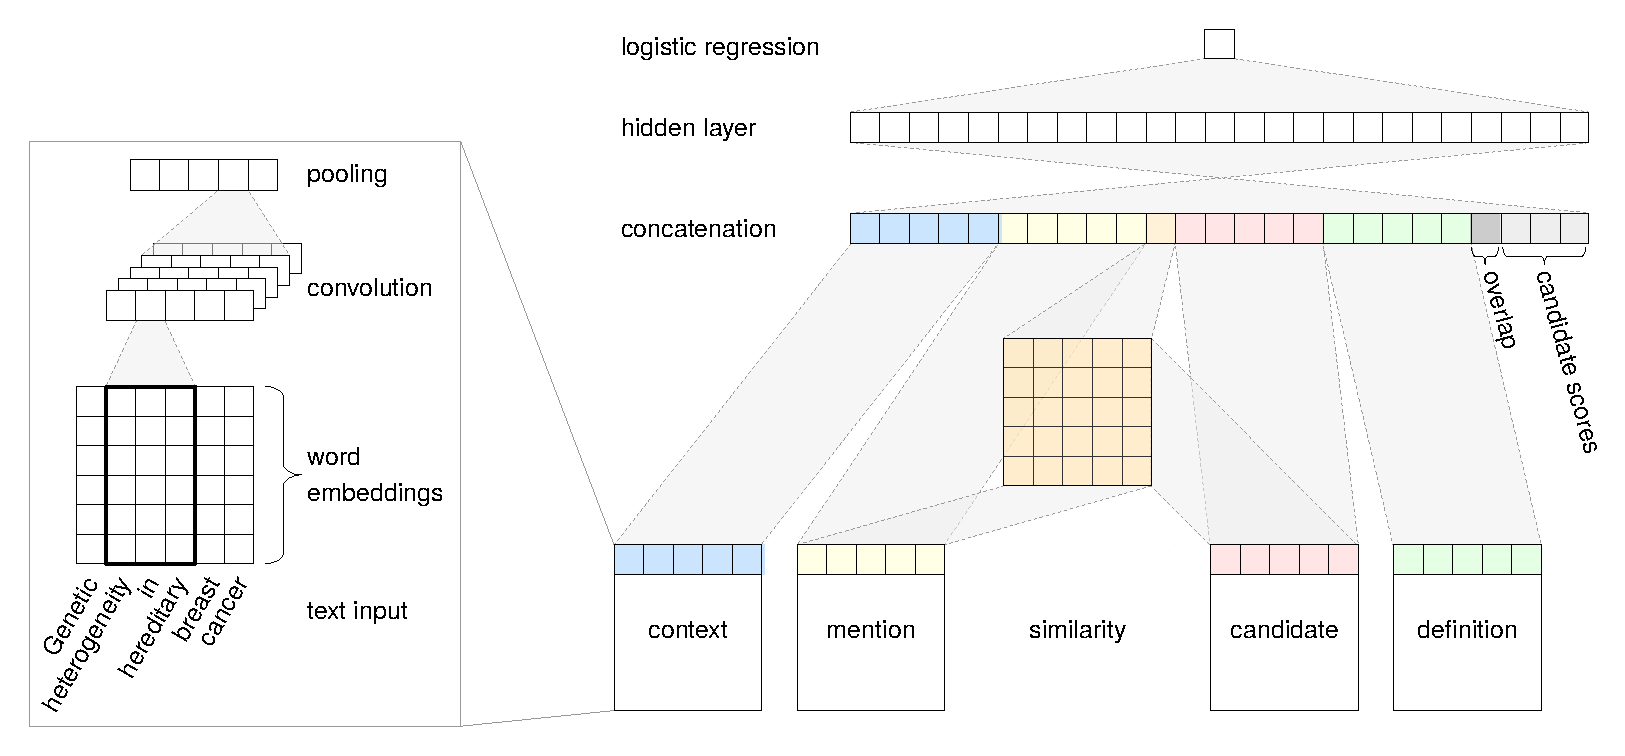
\includegraphics[width=\textwidth]{img/nn-arch.pdf}}
\caption{Architecture of the CNN used for ranking candidate names.}\label{fig:sys-arch}
\end{figure*}

Figure~\ref{fig:sys-arch} shows the architecture of the CNN.
During training and prediction, each mention-candidate pair is a separate data point.
As its input, the network considers four textual units:
the current mention, the current candidate name, the context of the current mention (\ie the complete abstract/report), and a dictionary definition of the candidate concept (serving as an equivalent of the mention context).

All textual units -- mention, candidate, context, definition -- share the same semantic representation in the network.
At the word level, the texts are embedded using pretrained word vectors.
We used the vectors trained on PubMed abstracts by \cite{chiu-et-al:2016:BioNLP} with a context window of 30 tokens,  % NB: Chiu et al say win-2 worked better for NER, but win-30 worked better here (mention in footnote?)
and applied padding to ensure fixed-length input sequences across all samples.
In the subsequent network layer, a convolution operation is applied to capture informative word n-grams.
We used different filter widths ($n \in {2,3,4}$) with 50 kernels each.
% TODO: mention tanh activation
Using 1-max pooling, the most informative feature of each kernel is extracted.
The pooled values form a feature vector carrying semantic information about the respective textual unit.

The semantic representations of all four text inputs are concatenated in the subsequent layer, together with a node each for semantic and lexical similarity as well as the scores from candidate generation.
The semantic similarity is determined by a dedicated layer for joining the semantic representations of the mention and candidate name with a weight matrix that is updated during training.
The lexical similarity is calculated as the Jaccard index  % TODO: reference
between the stemmed word tokens \citep{porter:1980} of the mention and candidate name.

The nodes of the concatenation layer are fully connected to a hidden layer of the same shape.
The scoring task is modeled as a logistic regression problem, using a single output node with sigmoid activation and binary cross-entropy loss.
% TODO: mention (and cite) optimizer?

\subsubsection{Identifier mapping}
\label{ssub:id-mapping}

Finally, the scored candidate names need to be mapped to terminology identifiers.
For each mention, the best-scoring name is determined and looked up in the terminology.
In the majority of the cases, this procedure is straight-forward, as most of the synonym names are unambiguous.  % TODO: give actual figures for both terminologies
However, if the top-ranking name maps to multiple concepts, the remainder of the ranked list is searched for disambiguation cues using the following heuristic:
\begin{enumerate}
  \item\label{enum:start} Consider the next-lower scoring candidate name $c$ and determine the set of identifiers $I_c$ to which it maps.
  \item Compute the intersection of $I_c$ with $I_t$, the identifiers of the top-scoring candidate. If $I_c \cap I_t$ is empty, repeat from Step~\ref{enum:start}.
  \item Set $I_t \leftarrow I_c \cap I_t$. If there is still ambiguity, \ie if $|I_t| > 1$, repeat from Step~\ref{enum:start}.
\end{enumerate}
If this procedure does not fully disambiguate the candidate name, we make an arbitrary, deterministic decision.
% TODO: report the number of amibiguous predictions for each dataset
% TODO: analyse how well this heuristic works

% TODO: mention threshold for NIL symbol (not used)?



\section{Results}

We trained and optimized our system using the given training sets.
For validation during development, we used the predefined development set for the NCBI disease corpus; for the ShARe corpus, we separated a validation set of 50 reports (25\,\%) from the training set, using stratified sampling to ensure a similar distribution with respect to document length and report type.
Final evaluation was performed on the respective test sets.

% TODO: is this in the right place?
The optimal configuration for both datasets was almost identical.
For the NCBI disease corpus, we used a filter width of 3 tokens in the convolution, whereas the ShARe corpus benefitted from using a combination of filter widths 2, 3 and 4.
The candidate generator for composite mentions was disabled for the ShARe corpus, as this type of annotation only occurs in the NCBI disease corpus.

After finalizing hyper-parameter tuning, we performed an additional evaluation with an ensemble setting.
We divided the training data of the ShARe corpus into five portions, using each of them to validate a separate model which was trained on the concatenation of the remaining four.
All five models are then applied to the test set, in that the scores for each candidate name are averaged before ranking.
We performed an analogous evaluation with the NCBI disease corpus, using a 7-fold division.

Table~\ref{tab:results} summarizes the results of our system compared to the state of the art.
The figures denote linking accuracy, \ie the proportion of correctly predicted identifiers given ground-truth mention spans.%
\footnote{For the NCBI disease corpus, alternative IDs listed in the same MEDIC concept were considered equivalent to the main ID.}  % This is how TaggerOne was evaluated, as Robert Leaman told me by email.
For both datasets, using an ensemble system produces better results than relying on a single train/development split.
With an accuracy of 88.75\,\%, our system performs similarly to TaggerOne, which has the highest linking score published for the NCBI disease corpus so far.
For the ShARe corpus, we were able to improve over the previously reported approaches, reaching 92.41\,\% accuracy.

\begin{table}[!t]
\processtable{Linking accuracy of our systems (context-CNN) and other approaches reported in the literature\label{tab:results}}
{\begin{tabular}{@{}lll@{}}\toprule
                                   & NCBID  & ShARe \\\midrule
  context-CNN, single model        & 0.8813 & 0.9187 \\
  context-CNN, ensemble            & 0.8875 & 0.9241 \\
  \cite{liu-xu:2018:NLPCC}         & 0.853  & -- \\
  \cite{lihaodi-et-al:2017}        & 0.8610 & 0.9030 \\
  TaggerOne                        & 0.888  & -- \\
  \cite{dsouza-ng:2015:ACL-IJCNLP} & 0.8465 & 0.9075 \\
  DNorm                            & 0.8220 & -- \\\botrule
\end{tabular}}{Single model: trained with the predefined train/development split for NCBID and a stratified 3:1 split for ShARe. Ensemble: $n$ models (NCBID: 7, ShARe: 5) trained on $n$ folds over the training+development set.}
\end{table}



\section{Discussion}

\begin{table}[!t]
\processtable{Ablation experiments: reduced systems with one or more components removed (test-set accuracy, best of two runs)\label{tab:ablation}}
{\begin{tabular}{@{}lll@{}}\toprule
                                    & NCBID  & ShARe \\
  \midrule
  full system                       & 0.8813 & 0.9187 \\
  \midrule
  $\neg$context                     & 0.8531 & 0.9168 \\
  $\neg$definition                  & 0.7646 & 0.8191 \\
  \midrule
  $\neg$similarity                  & 0.8563 & 0.9152 \\
  $\neg$similarity, $\neg$mention   & 0.8385 & 0.8866 \\
  $\neg$similarity, $\neg$candidate & 0.8500 & 0.8910 \\
  \midrule
  $\neg$all CNNs                    & 0.7208 & 0.6550 \\
  \botrule
\end{tabular}}{}
\end{table}

We performed an ablation study in order to analyse the contribution of the individual inputs to the model.
As shown in Table~\ref{tab:ablation}, we ran a series of experiments, where certain components of the system were disabled in turn.
In each run, the semantic representation (embedding, convolution, and pooling layers) of one or more textual units was removed from the architecture, thus reducing the size of the concatenation layer.
The results reveal that every component contributes to the total performance, even though the decrease in accuracy is only marginal in a few cases.
The two datasets show varying degrees of performance loss when removing individual components.
However, the ordering is almost identical: both the NCBI disease and the ShARe corpus suffer the most from omitting all semantic representations, followed by disabling the definitions, while the smallest drop is observed for skipping similarity or context (with a very small respective difference).
The most interesting observation is the outstanding role of the dictionary definitions, while the context of the disease mention is of subordinate importance.


analyse contribution of context (kernel inspection)

maybe analyse contribution of individual candidate generators (another ablation series)?

any differences between text genre?

ambiguity in candidate names\dots

explain and regret need for candidate generators

future work: doing hierarchical classification (producing the IDs directly) would be cool. something like \cite{guo-et-al:2018} looks interesting, but how to deal with the problem that we will never have training examples for 10k (not just 100) labels?



\section*{Acknowledgements}

Submission guidelines:
Please ensure you acknowledge all sources of funding.
Details of all funding sources for the work in question should be given in a separate section entitled 'Funding'. This should appear before the 'Acknowledgements' section.

But: the template and published examples list funding later.
Nobody acknowledges source of funding.
\vspace*{-12pt}



\section*{Funding}

This work was supported by \dots

An example is given here: ‘This work was supported by the National Institutes of Health [AA123456 to C.S., BB765432 to M.H.]; and the Alcohol \& Education Research Council [hfygr667789].’
\vspace*{-12pt}



\bibliographystyle{natbib}
\bibliography{refs}


\end{document}
